\documentclass{article}
\usepackage[round]{natbib}
\usepackage{amsmath,amssymb,amsfonts, bbm}%
\usepackage{geometry}%
\usepackage{color}
\usepackage{graphicx}
\usepackage{authblk}
\usepackage{nameref}
\usepackage[right]{lineno}
\usepackage{subcaption}
\usepackage{tikz}
\usepackage{placeins}
\usepackage[hidelinks]{hyperref}

\newcommand{\tsinfer}[0]{\texttt{tsinfer}}
\newcommand{\kwarg}[0]{\texttt{KwARG}}
\newcommand{\argneedle}[0]{\texttt{ARG-Needle}}
\newcommand{\argweaver}[0]{\texttt{ARGweaver}}
\newcommand{\argweaverD}[0]{\texttt{ARGweaver-D}}
\newcommand{\relate}[0]{\texttt{Relate}}
\newcommand{\espalier}[0]{\texttt{Espalier}}
\newcommand{\arbores}[0]{\texttt{Arbores}}
\newcommand{\tskit}[0]{\texttt{tskit}}
\renewcommand{\deg}{\mathrm{deg}}
\newcommand{\comment}[1]{{\it \color{orange} (#1)}}

% Bold the 'Figure #' in the caption and separate it from the title/caption with a period
% Captions will be left justified
\usepackage[aboveskip=1pt,labelfont=bf,labelsep=period,justification=raggedright,singlelinecheck=off]{caption}
\renewcommand{\figurename}{Fig}

% deal with supplementary items
\newcommand{\supplementarysection}{%
  \setcounter{figure}{0}% Reset figure counter
  \let\oldthefigure\thefigure% Capture figure numbering scheme
  \renewcommand{\thefigure}{S\oldthefigure}% Prefix figure number with S
  \section{Supplementary section}% Set supplementary section
}

% adjust inter-paragraph spacing - this one's for you, Gertjan
\setlength{\parskip}{0.5\baselineskip}

\begin{document}

\linenumbers
\title{Computing likelihoods under the SMC for a general class of ARGs.}

% First authors
\author[1, $\dagger$]{Gertjan Bisschop}
\author[1]{Jerome Kelleher}
% last author
\author[3]{Peter Ralph}

\affil[$\dagger$]{Denotes corresponding author}

\maketitle

\affil[1]{Big Data Institute, Li Ka Shing Centre for Health Information and Discovery, University of Oxford, OX3 7LF, UK}
\affil[2]{Department of Statistics, University of Oxford, OX1 3LB, UK}
\affil[3]{University of Oregon, USA}

\begin{abstract}
There currently is no way to connect the output of the diverse
range of ARG inference methods back
to a model that would allow us to perform a probabilistic exploration of the
ARG space around the point estimate, or likelihood-based inference.
\end{abstract}

\section{Introduction}
Following recent breakthroughs in simulation and inference methods,
there is now intense interest in applying Ancestral Recombination Graphs (ARGs)
to a variety of questions in evolutionary
biology~\citep{lewanski_era_2024,brandt_promise_2024}.
ARGs describe the intricately linked paths
of genetic inheritance resulting from
recombination~\citep{hudson_properties_1983,griffiths_ancestral_1996,wong_general_2023},
and contain rich detail about ancestral processes.
% TODO rephrase this a bit, would be a lot of duplication of references
% in the current formulation.
Applications using inferred ARGs as input have begun to
appear~\citep{osmond_estimating_2021,
fan_genealogical_2022,
hejase_deep_2022,
guo_recombination-aware_2022,
zhang_biobank-scale_2023,
nowbandegani_extremely_2023,
ignatieva_distribution_2023,
fan_likelihood_2023,
huang_estimating_2024}.
Additionally, there is a rich suite of tools growing around
the \texttt{tskit} ARG library~\citep{ralph_efficiently_2020}
including simulation~\citep{kelleher_efficient_2016,kelleher_efficient_2018,
adrion_community_2020,terasaki_geonomics_2021,
baumdicker_efficient_2021,
korfmann_weak_2022, petr_slendr_2023,tagami_tstrait_2024},
ARG inference~\citep{kelleher_inferring_2019,speidel_method_2019,
wohns_unified_2022,mahmoudi_bayesian_2022,
rasmussen_espalier_2022,
zhang_biobank-scale_2023,zhan_towards_2023} and analysis
packages
% etc
\citep{nowbandegani_extremely_2023,fan_likelihood_2023}.
Infererence methods now tend to fall into two classes: those that
sample from a statistical
% TODO add SINGER
model~\citep{rasmussen_genome-wide_2014,hubisz_mapping_2020,mahmoudi_bayesian_2022}
or parsimony~\citep{ignatieva_kwarg_2021,rasmussen_espalier_2022},
and those based on
heuristics~\citep{kelleher_inferring_2019,speidel_method_2019,
zhang_biobank-scale_2023}.
Typically, the more rigorous approaches can handle 10-100 samples,
while the approximate methods can scale to 10s to hundreds of
thousands of samples. With the explosive growth in dataset
sizes in recent years~\citep[e.g.][]{bycroft_genome_2018,halldorsson_sequences_2022,
all_genomic_2024} there is a pressing need for more statistical
rigor in large scale ARG inference.

Perhaps the clearest route to statistical rigor is through scalable
model-based inference, a central element of population genetics.
The coalescent~\citep{kingman_genealogy_1982,kingman_coalescent_1982,hudson_testing_1983,
tajima_evolutionary_1983} has proved to be a useful model, and is the
basis of a wide variety of inferences [some citations, e.g Hey IM model]. 
The incorporation
of recombination in the coalescent process~\citep{hudson_properties_1983}
has proved to be much more difficult.
% FIXME rephrase, next two sentences, lifted from ARG paper
Early work on inference under the coalescent with recombination
focused on the problem of
inferring the parameters of the
stochastic process, where the ancestry was regarded as a
latent parameter to be averaged out
\citep[e.g.][]{griffiths_ancestral_1996,kuhner_maximum_2000,
nielsen_estimation_2000,
fearnhead_estimating_2001}.
% TODO reuse some of the ideas from the SMC paper here, it has
% some good explanations.
These methods met with limited success
because the state space of ARGs is overwhelmingly large, and
lacks a simple geometry or neighbourhood structure for inference or
sampling methods to  exploit.
The introduction of the Sequentially Markovian Coalescent (SMC)
approximation to the coalescent with recombination
by~\cite{mcvean_approximating_2005} was a seminal contribution,
and has made many different inferences
% TODO add some more recent stuff
feasible~\citep[e.g.]{li_inference_2011,paul_accurate_2011,schiffels_inferring_2014}.
In particular, the SMC is the basis for ARG sampling methods
like ARGweaver~\citep{rasmussen_genome-wide_2014}, which remains the
% TODO list other places ARGweaver has come out on top in terms of accuracy.
gold-standard in terms of accuracy~\citep{brandt2022evaluation}

% THE PROBLEM!!! OMG it's terrible!!!
Although major breakthroughs in scale have been achieved by hueristic
ARG inference
methods~\citep{kelleher_inferring_2019,speidel_method_2019,zhang_biobank-scale_2023},
these methods are currently fundamentally incompatible with rigorous
inference under population genetic models such as the SMC. This is 
because these methods return approximate ARG
\emph{structures}~\citep{wong_general_2023} [WEAK, FIXME]. Specifically,
we cannot evaluate a likelihood of these ARGs in coalescent 
models under the classical 
\cite{kuhner_maximum_2000} formulation, as these formulations assume
that complete information about recombination events is present.
[NOTE the following is super weak, and needs a lot of work.]
This inability to connect the results of large-scale inference methods
with a generative model
is a fundamental limitation, and limits both the utility of 
current point estimates as well as the possibilities for further
inference. Specifically, we are unable to quantify uncertainty 
around heuristic point estimates. We cannot explore ARG space
around the point estimates using (e.g. MCMC), as we have no way definition
of improvement. We cannot compare models of demography, or evaluate the 
goodness of fit for model estimates.

%% This is how we solve it
[TODO figure out the gARG, tree sequence etc mess]
Here, we bridge this gap between models and the products of approximate
inference by defining a likelihood function for any 
``genome ARG''~\citep{wong_general_2023} under the SMC. Using a novel
formulation of the SMC that focuses on the contributions of nodes and 
edges [FIXME] in a backwards-in-time way, we provide an efficient 
algorithm that can compute a likelihood for any gARG under this model.
We demonstrate the flexibility of this approach by XXX, and show
[SOMETHING]. 


%%%%%%%%%%%%%%%%%%%%%%%%%%%%%%%%%%%%
\section{Methods and Results}

First, we define the SMC process in a ``backwards-in-time'' way,
rather than the usual ``along-the-genome'' way.
Note that this is a
reiteration of the original work of \citet{mcvean_approximating_2005}.
Then, we describe
in more detail what sort of information we have in estimated ARGs.
In the subsequent section we connect the two and
show how the ``backwards-in-time'' description
makes it relatively straightforward to compute the likelihood
for a more general class of estimated ARGs.
Finally, we close with a demonstration that the likelihood computation can be used
to do Bayesian inference on ancestral population sizes.

% % % % % % % % % % % % % % % % % %
\subsection{SMC backwards-in-time}\label{par:description}

In its backwards-in-time formulation, the SMC \citep{mcvean_approximating_2005} only requires a
simple modification to the coalescent with recombination.
Instead of allowing any pair of lineages to coalesce,
the SMC is the process in which only lineage with \emph{overlapping} genomic intervals may coalesce.
Surprisingly, although this is defined in terms of a backwards-in-time Markov process,
the resulting tree-valued process along the genome is also Markov.
Although \citet{mcvean_approximating_2005} verbally described the SMC 
using this backwards-in-time description, their analysis
was almost entirely in left-to-right terms,
and subsequent papers followed this trend 
\citep{li_inference_2011,paul_accurate_2011,schiffels_inferring_2014,rasmussen_genome-wide_2014}.

We now define the process more formally,
and following the notation of \citet{mcvean_approximating_2005}.
At any point in time, the state of the process is $L(t)$,
the set of labeled lineages extant at time $t$,
where each ``lineage'' is represented by a half-open interval
which represents the ancestral material carried by that lineage,
and labeled by an integer.
So, we can write $L(t) = \{X_i(t)\}_{i=1}^{n(t)}$,
where the $i^\text{th}$ lineage is $X_i(t)$
and is of the form
$X_i(t) = [x_{i}, y_{i})$,
for some interval endpoints $x_{i} < y_{i}$.
The \emph{size} of the interval is $|X_i(t)| = y_{i} - x_{i}$.
Since we look backwards in time, $t=0$ is today, and so
$L(0)$ consists of $n$ sampled lineages, labelled $0$ to $n-1$,
each represented by a single interval spanning the entire genome.
Then, the process evolves by a succession of coalescence and recombination
events until each segment of ancestral material is only present in one lineage.
The waiting time to next event is determined by these two competing processes
with exponentially distributed waiting times as outlined below.

Recombination is described by a Poisson process of rate $r$ per unit of genomic length and time:
so, if $T(t) = \sum_i |X_i(t)|$ is the sum of the total sizes of all lineages,
then recombination occurs at instaneous rate $rT(t)$.
A recombination to the left of $x$
(i.e., between base pairs $x$ and $x-1$)
with $x>x_{i}$ and $x<y_{i}$ splits lineage $i$ into two new lineages,
which each are given new, unique labels
(and lineage $i$ is removed).
This operation keeps the total amount of ancestral material unchanged.

Coalescence occurs between
two overlapping lineages at rate $\lambda = 1/(2N_e)$
(if we assume a randomly mating, diploid population of constant size $N_e$).
The newly formed lineage acquires the union of both ordered intervals, % L is updated accordingly
and the original lineages are removed.
Although coalescence is reciprocal, here we'll define a strict total order
on all lineages in $L(t)$ based on their leftmost starting points (and index to break ties).
For any such strict total order,
the instantaneous rate of coalescence then equals $\lambda$ multiplied by the number of overlapping pairs,
i.e., $\lambda \sum_{i \neq j} I_{ij}$,
where
\begin{equation} \label{def:coal}
I_{ij} = \begin{cases}
    1 & X_i > X_j \text{ and } s(X_i) \cap s(X_j) \neq \emptyset \\
    0 & \text{otherwise.}
\end{cases}
\end{equation}
We say that lineage $j$ can coalesce \emph{into} lineage $i$ if $I_{ij} = 1$
(and notice that if $I_{ij} = 1$ then $I_{ji} = 0$).

For future use, define $C_i(t)$ to be the set of lineages that can coalesce into lineage $i$,
i.e., $C_i(t) = \{X_j \in L(t) | I_{ij}(t) = 1\}$.
(Therefore, $|C_i(t)| = I_{i}(t) = \sum_{j} I_{ij}(t)$,)
and the total rate of coalescence at time $t$ is $\sum_{i} |C_i(t)|$.) 
Because $I_{ij}$ is defined in terms of a total order, the sets $C_i(t)$ are disjoint,
which will simplify the likelihood computations.
In particular,
although recombination affects \emph{which} lineages can coalesce into $i$,
it does not change the \emph{number} of such lineages:
in other words, a recombination event changes $C_i(t)$ but not $I_{i}$.
Another useful quantity to know is the number of lineages carrying material
at each point on the genome:
for a location $z$ and time $t$, this is
\begin{equation}
    N(t,z) = \#\{i : z \in X_i(t) \} .
\end{equation}

Finally, there is one more operation that allows the process to terminate:
portions of the edges of lineages that have entirely coalesced
(i.e., that are ancestral to all samples) are removed.

Formally, after any coalescence or recombination event,
the segment $[x,y)$ carried by the lineage
is replaced by the largest (pair of) segment(s) whose endpoints have not
coalesced, i.e., $x$ is replaced by $\min\{ z \ge x : N(t,z) > 1\}$,
and $y$ is replaced by $\sup\{ z \le y : N(t,z) > 1\}$.
By reasoning about the process in this way we can keep representing 
all lineages by means of a single half-open interval throughout.

\comment{Adapt figure to represent this}

% % % % % % % % % % % % % % % % % %
\subsection{Estimated ARGs} \label{par:recording}

Although the term Ancestral Recombination Graph (ARG) has been used to mean several things,
in the generic sense, it is a labeled graph structure that records
the inheritance of genetic material \citep{wong_general_2023}.
An ARG of the sort we consider describes the history of inheritance
of the genomic material of a focal set of individuals (that we call \emph{samples}).
Concretely, an ARG is equivalent to a collection of (non-contradictory) statements
of the form ``$c$ inherited from $p$ on the genomic segment from $\ell$ to $r$'',
where $c$ and $p$ are (haploid) genomes, and $\ell$ and $r$ are genetic coordinates.
We record each such statement in an ``edge'',
often summarized as the tuple $(p,c,\ell,r)$.
By ``describes the history'',
we mean that each node in the ARG represents a specific (ancestral) genome,
and that the ARG specifies the genealogical tree describing how the samples are related
at each point on the genome.

So, an ARG can be thought of either as a collection of inheritance relationships
between ancestral haplotypes,
or as a sequence of genealogical trees that have common node labels.
Fig.\ref{fig:smc-unary} shows a small ARG
that describes relationships between four samples on a 100bp piece of genome,
represented as both a graph (top) and a series of local trees (bottom).
Both structures represent the same information:
for instance, the fact that the ancestral genome at $a$
inherited the left half of its genome from ancestor 6
and the right half from ancestor 5
is seen in the fact that the first two trees have $a$ below 6,
and the remaining have $a$ below 5.
The blue dotted line from $a$ in the second tree to 5 in the third tree
draws our attention to the fact that
the path traced by $a$'s ancestry switches at that point.
In fact, $a$ is in blue because it is a \emph{recombination} node --
\comment{wait is it ``recombination node'' or ``recombinant node''?}
an ancestor that has a segment of genome inherited by a sample,
but that segment was inherited in two pieces from their parent.
Other nodes (labeled by black numbers) are either samples
or \emph{coalescence} nodes --
ancestors that are the most recent common ancestor for two samples
at some place along the genome.

Crucial for the equivalence between both representations is the presence of
nodes that only have a single child along one or more local trees --
i.e., are \emph{locally unary}.
Recombination nodes (in blue) have a single child in all trees.
However, coalescent nodes can be locally unary as well:
for instance, sample 3 inherited a longer stretch of genome from ancestor 5
than did sample 2.
In the top plot, this is visible because the pink bar below node 5
extends further to the left than does the blue bar,
while in the bottom plot, this is visible because node 5 is parent to 3
in the second tree, but not to node 2, and so is unary.

A key observation of \citet{mcvean_approximating_2005}
was that the sequence of trees along the genome
generated by the SMC was Markovian \emph{after removing all unary nodes}.
In other words, if we remove recombination nodes entirely,
and erase the unary portions of coalescent nodes,
then the distribution of the next tree can be generated only knowing the current tree.
(To see that the unary nodes makes the process non-Markov,
consider that a node in a tree might be unary either because it's about to be a coalescent node
or it already has been:
looking at the second tree, we know node 5 will be coalescent further down the sequence
because it was not present in the first tree.
So, the first tree gives us information about subsequent trees
that the second tree alone could not.)
However, removing these unary portions of nodes seems odd
when one considers the consequences in the haplotype inheritance graph
of the top figure.
As pictured, both figures tell us that
3 inherits the middle bit of the genome from 7 through 5.
However, if we erase 5 from the second tree,
does this suggest that 3 inherited a single segment from 7 along two distinct paths?
The haplotype inheritance graph above makes it clear that this is unlikely:
it is in fact reasonable to leave in these unary sections.

Furthermore, these unary nodes enable
us to uniquely identify all lineages that were hit by a recombination event,
even if we simplify the ARG by removing all recombinant nodes
($a$, $b$, and $c$ in Fig.\ref{fig:smc-unary}).
In the absence of these recombination nodes, a recombination can be observed
easily enough as a change in parent going from one genomic region to the next.
Without the recombination nodes we no longer know the precise time of each recombination event,
but we do still have constraints on the time:
for instance, we know that $c$ happened somewhere between node 5 and node 7.
More generally, a recombination node must happen somewhere between the child node
and the most recent of the parent nodes.
This is again easier to visualise using the
graph representation (blue shaded area, fig.\ref{fig:smc-unary}).
Although these unary nodes are useful and to some degree clearly inferrable,
they are not always represented by simulators or ARG reconstruction methods.
However, to our understanding this is because
the field is used to thinking in terms of the trees
rather than in terms of relationships between haplotypes,
not because of any question of knowability.
Currently,
\argweaver{} \citep{rasmussen_genome-wide_2014}
\tsinfer{} \citep{kelleher_inferring_2019}, and
\kwarg{} \citep{ignatieva_kwarg_2021}
estimate ARGs including unary portions of coalescence nodes.
However, it is unclear to what degree these are well-inferred,
as most evaluation of inferred ARGs thus far has focused on marginal trees
(e.g., \citet{brandt2022evaluation,kelleher_inferring_2019},
but see \citet{deng2021distribution})
and thus completely ignore such unary nodes
(and their implications for inherited haplotypes).

In the next section we will derive an expression to compute the
likelihood for an ARG under the SMC for which we have no information on the
time to any of the recombination events. We will then detail an algorithm
that allows us to efficiently compute this value by iterating over the local trees.
To do this, we will rely on the unary nodes
to identify each lineage involved in a recombination event
as described in this section.


\begin{figure}[!ht]
\centering
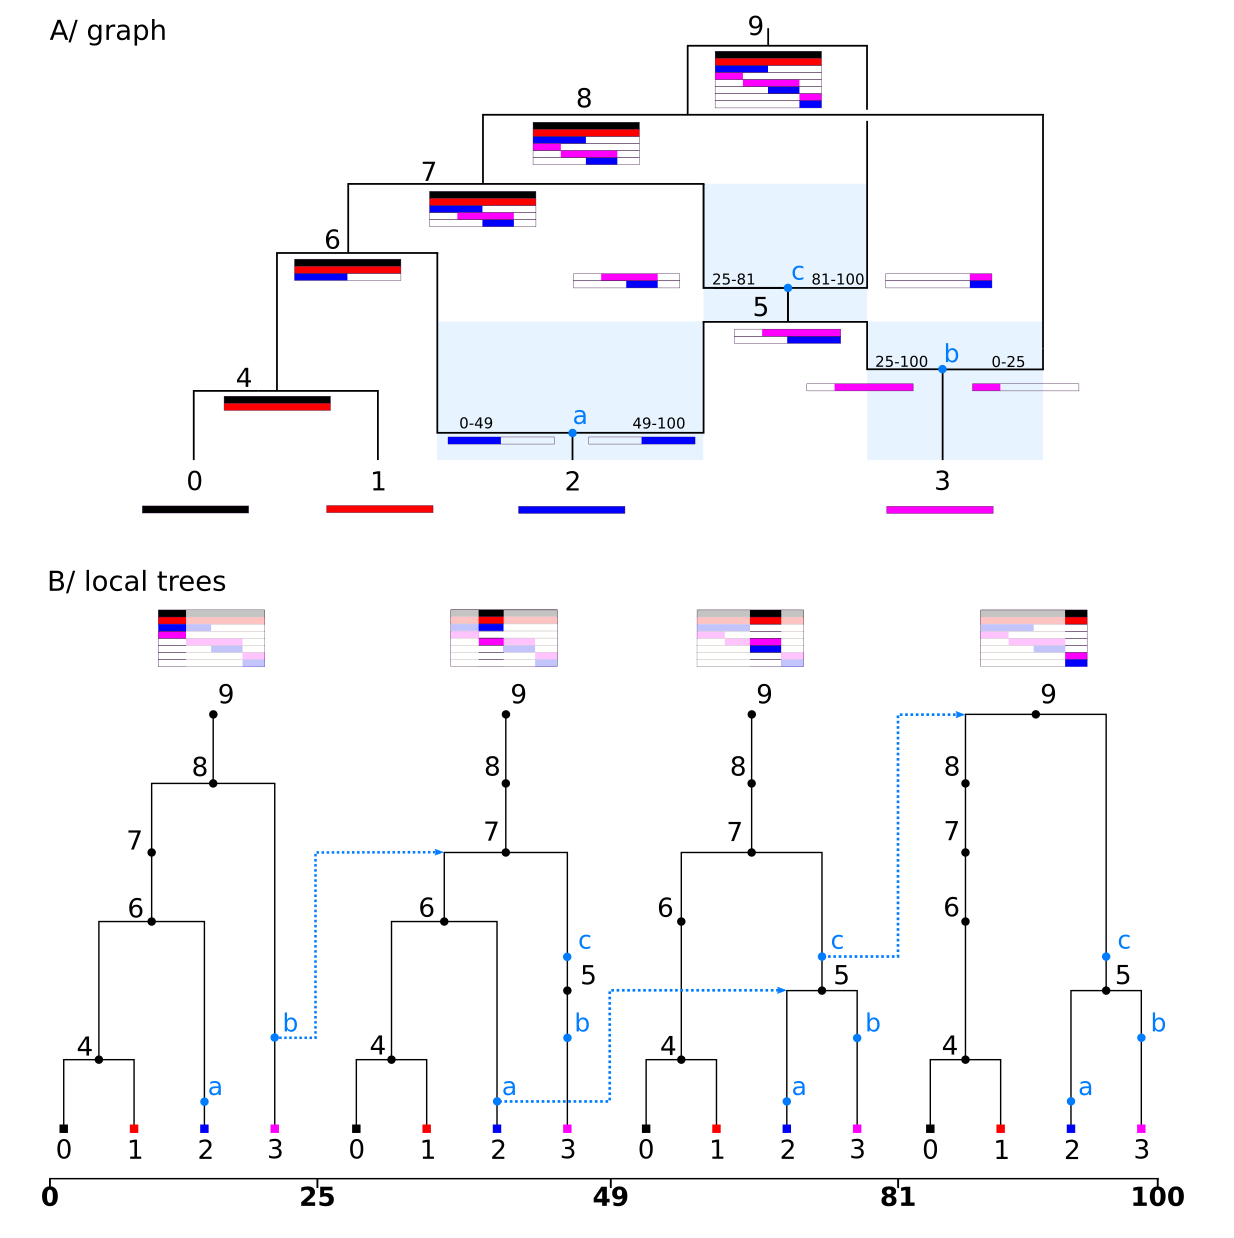
\includegraphics[width=\textwidth]{figures/smc_custom_2rows_area_full_hap.png}
\caption{ARG (top) generated under the SMC and its representation as a
series of local trees (bottom). To ensure the one-to-one correspondance
between both representations a node is recorded for each local tree whenever
a node is encoundered along its ancestry path in the graph representation.
This results in nodes that (locally) have only a single child, and are therefore
(locally) unary. Blue (unary) nodes represent recombinant nodes.
The blue arrows shows the familiar left-to-right logic of the SMC whereby
the floating lineage coalesces randomly
with a the remaining portion of the local tree following recombination.
Note how the presence of the unary node on a local tree is
indicative of either a past (to the left of the local tree)
or future (to the right) coalescence event.
Both ARG representations can be simplified by removing the recombinant nodes.
In that case the information we have on the time to each of these events is
limited to the windows (blue shaded array) delimited by by the age of
the child node $c$ associated with that lineage and the minimum age of
the parents of the edges connecting to $c$.
}
\label{fig:smc-unary}
\end{figure}



% % % % % % % % % % % % % % % % % %
\subsection{Calculating likelihoods} \label{par:liks}

The process of recombination only affects one lineage at a time
(and does not even depend on the state of other lineages).
On the other hand, coalescence events necessarily involve more than one lineage.
However, the asymmetric way we define coalescence above
allows us to uniquely associate each event with a single lineage,
which allows us to cleanly factor the likelihood across edges and nodes.
The data structure we will compute the likelihood of
is a collection of \emph{edges} $E$,
where each edge $e$ is of the form $e = (p,c,x,y)$.
Recall that this means that node $c$ inherited genetic material from node $p$
over a region with span from $x$ to $y$ along the genome
(see Figure~\ref{fig:likelihood}).
So, $x$ and $y$ are genomic coordinates,
while $c$ and $p$ are in $N$, the set of \emph{nodes}
(i.e., distinct sampled or ancestral haplotypes).

We have defined the SMC process in terms of rates of various types of events.
In general, the likelihood for a continuous-time Markov process specified in this way
is $\exp(-\Lambda) \prod_i \lambda_i$,
where $\lambda_i$ is the rate of the $i^\text{th}$ realized event,
and $\Lambda$ is the sum of all rates of all possible events
integrated over the entire process
(also called the ``total hazard''). \comment{if we want to spell it out even further:
Note that the time to the next event is distributed as $\Lambda \exp(-\Lambda)$. And
the probablility that the next event is of type $i$ is $\lambda_i / \Lambda$.}

The contributions to the likelihood from coalescent and recombination events
is straightforward, since each possible coalescence is associated with rate $\lambda$,
and each recombination with rate $r$.
Under the SMC, we only ever have two lineages coalescing at a time;
however, inferred ARGs may have more-than-binary mergers.
We treat these as if there were zero-length edges
between a sequence of mergers;
the order of these unresolved mergers does not affect the likelihood.
(Under the SMC the likelihood of a zero-length edge is zero;
but this is not special: since edge lengths are continuously distributed,
the likelihood of any particular value is also zero.)
Let $\deg_o(n) = \#\{e \in E : p_e=n\}$ be the out-degree of a node $n$,
i.e., the number of edges having $n$ as a parent.
Since mergers are binary in the SMC,
this must have been the result of $\deg(n) - 1$ coalescences,
and so this contributes a factor of $\lambda^{\deg_o(n)-1}$ to the likelihood
for nodes with any children.
Similarly,
let $\deg_i(n) = \#\{e \in E : c_e=n\}$ be the in-degree of a node $n$,
i.e., the number of edges having $n$ as a child.
Each additional edge that is ancestral to a given node
implies one additional ancestral recombination event,
and thus a factor of  $r^{\deg_i(n)-1}$ in the likelihood,
if the node has any parents.
Put together, these two contribute
\begin{equation}\label{eq:coal}
    \prod_{n \in N} \lambda^{\deg_o(n)-1} r^{\deg_i(n)-1}  
    =
    r^{|E|-|N|+n_r} 
    \lambda^{|E|-|N|+n_s} 
\end{equation}
to the likelihood,
where $n_r$ is the number of nodes with in-degree 0 (roots),
and $n_s$ is the number of nodes with out-degree 0 (usually, samples).
(The simple form follows because each edge contributes exactly one
to some node's out-degree and some node's in-degree.)


\begin{figure}
    \centering
    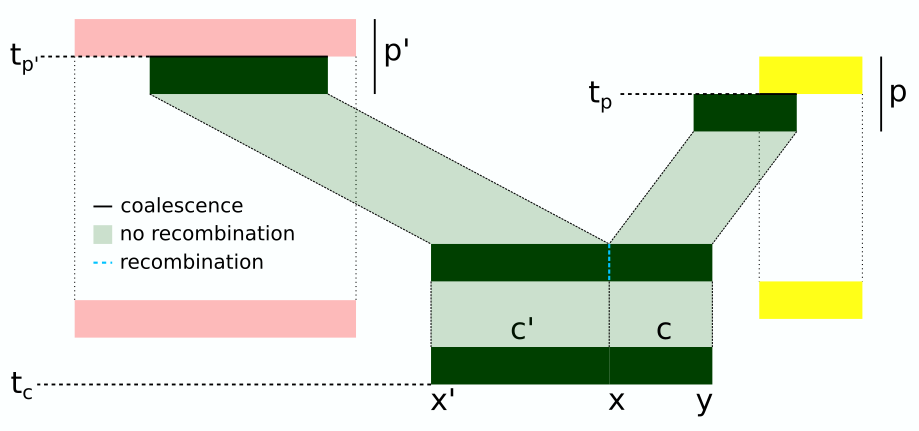
\includegraphics[width=\textwidth]{figures/single_event.png}
    \caption{
        Proposed figure to explain the likelihood computation with.
        TODO: change numbered labels to match the order in the text,
        add $x$ and $y$.
        \label{fig:likelihood}
    }
\end{figure}

Now consider the ``hazard'' associated with recombination.
Begin with an edge $e = (p,c,x,y)$.
This implies that there was a sequence of lineages
from the time of the child $c$ (call this time $t_c$)
back to the time of the parent $p$ (again, $t_p$),
that contained the segment $[x,y)$,
and the lineage that directly inherited from $p$
had the segment $[x,y)$.
Under the SMC,
we therefore know there was no recombination between $x$ and $y$
on any of the lineages 
over this time span,
the probability of which is
$\exp(-r \times A)$, where $r$ is the recombination rate
and $A$ is the total area (eligbile links times depth) of the edge.
So, the first contribution to the likelihood from this edge $e$ is
\begin{equation}\label{eq:span}
A_e(r) = \exp(-r (y-x - \mathbbm{1}_{x > x_c})(t_p - t_{c})) .
\end{equation}
Note that if a recombination did occurr, then the number of links not
affected by recombination is 1 less (see \ref{eq:depth}).

Finally, we turn to the hazard associated with coalescence.
To do this, we need only consider what happens along the left side
of each edge.
The instantaneous rate of coalescence of a lineage whose left endpoint is at $x$
at a given time is equal to $\lambda$ multiplied
by the number of earlier lineages that overlap $x$ at that time.
Recall that we define a total order on edges,
by ordering by left endpoint and breaking ties by child
(i.e., $(p,c,x,y) < (p',c',x',y')$
if $x<x'$, or if $x=x'$ and $c<c'$).
Using this total order, we can define
$I_e(t)$ to be the total number of earlier edges that overlap edge $e$
and are present at time $t$.
Then, the cumulative hazard for coalescence of edge $e$
between time $s$ and $t$ is given by $F(e, s, t) = \int_{s}^{t} I_{e}(u) du$.
If the edge $e = (p,c,x,y)$
is the leftmost segment of material inherited by node $c$
(e.g., the lefthand segment ancestral to node $c$
in Figure~\ref{fig:likelihood}),
then no recombination occurred along this edge and 
this edge simply contributes $\exp(-F(e,t_c,t_p))$ to the likelihood.
However, if the edge is \emph{not} the leftmost segment,
then it was initiated by a new recombination breakpoint,
and we need to integrate over possible times the breakpoint occurred.
If this is the case, there is another edge $(p',c,x',x)$ with the same child node,
immediately adjacent to the focal edge $(p,c,x,y)$.
The recombination event that split the two must have happened between $t_c$
and the smaller of $t_p$ and $t_{p'}$. Note that two events must have happened
between $t_c$ and $\min(t_p, t_{p'})$; taking all this into consideration,
the contribution to the likelihood here is
\begin{equation}\label{eq:depth}
B_e(r, \lambda) = \begin{cases}
    e^{-\lambda F(e, t_c, t_p)}
        & \qquad \text{if } x=x_{c} \\
    \int_{t_c}^{t_{p} \wedge t_{p'}} e^{- r s} e^{-\lambda F(e, s, t_{p})} ds
        & \qquad \text{if } x>x_{c} ,
\end{cases}
\end{equation}
where $x_c$ is the leftmost position of the edges whose children are $c$.

% In that case $x=x_{c0}$ and $c$ did not coalesce until $t_p$.
% Alternatively, $x$ can be a new recombination break point that
% occurred on the lineage represented by $c$ at some time $s$ between $t_{c}$
% and $\min(t_p, t_{p^{\prime}})$, where $p^{\prime}$ is the parent of the
% edge $(c, p^{\prime}, X_{cp^{\prime}})$ ending at $x$. The new lineage formed
% by the recombination event and starting at $x$ can be given a temporary label
% $c_s$. In both cases, the cumulative hazard of a lineage $a$ coalescing
% between time $s$ and $t$ is given by $F(c, s, t) = \int_{s}^{t} I_{c}(u)du$
% such that:

%\comment{This is the old equation; I think the $e^{-rs}$ should not be there,
%    since it's already taken into account by \eqref{eq:span}.
%    Plus, the $\lambda$ and $r$ factors are now elsewhere.}
%\begin{equation}\label{eq:depth_old}
%B_{(c, p)}(\theta) = \begin{cases}
%e^{-\lambda F(c, t_c, t_p)} \lambda^{I_{cd}(t_p)} & x=x_{c0} \\
%\int_{t_c}^{t_{p} \wedge t_{p^{\prime}}} r e^{-rs} e^{-\lambda F(c_s, s, t_{p})} ds \lambda^{I_{c_{s}d}(t_p)} & x=x_{c_{s}0}>x_{c0} \\
%\end{cases}
%\end{equation}
%\comment{Do we still need this bit?}
%Here, the (second) exponential term gives the probability of not observing a
%coalescence event before $t_p$. In case of a recombination, $re^{-rs}$ further
%gives the probability of observing a recombination
%at time $s$ given a Poisson process along position $x$ with rate $r$.
%The time of the recombination is integrated out.
%The last term gives the point probability density of the coalescence event
%that terminates the edge. The indicator function is used to resolve
%the non-reciprocal nature of coalescence events as defined in \ref{def:coal}.

The likelihood of ARG defined by the set of edges $E$ and nodes $N$
given parameters $\theta$ then is
\begin{equation}\label{eq:full-lik}
    \mathcal{L}(\mathcal{G}|r, \lambda)
    =
    (r)^{|E|-|N|+n_r} (\lambda)^{|E|-|N|+n_s} \prod_{(c, p) \in E} A_e(r) B_e(r, \lambda) .
\end{equation}

% Although the first two factors are easily expressed in terms of numbers of edges and nodes,
% we will see below
% that in practice it is convenient to absorb these terms into per-edge contributions.

% refer to the algorithm in the supplements, briefly mention scalability
This likelihood expression is not only linear in the number of edges. An algorithm
(see supplementary information \ref{par:algo}) can be devised to efficiently keep
track of $I_e(t)$ by means of existing \texttt{tskit} functionality.
Note that we can accommodate for stepwise changes in the coalescence rate (or recombination rate)
through time by intersecting the internode intervals with the rate change intervals. 
Rate changes along the genome can be incorporated similarly.
Finally, we have only considered the topology and branch length information of any ARG.
Extending this expression by adding the likelihood of observing a set of mutations
given an ARG is given by

\begin{equation}\label{eq:lik-mut}
    \mathcal{L}(\mathcal{D}|\mathcal{G}, \mu)
    =
    \frac{1}{\mathcal{M}!} \prod_{(c, p) \in E} e^{-(y-x)(t_p-t_c)\mu^{|m_e|}} .
\end{equation}
where $\mathcal{M}$ the total number of mutations and $m_e$
the number of mutations along edge $(c,p)$ \citep{mahmoudi_bayesian_2022}.

% % % % % % % % % % % % % % % % % %
\subsection{Flexibility}

% likelihood surface
The last paragraph aims to highlight the flexibility of this approach 
and the impact of the various
degrees of completeness of the ARG on the likelihood.
Note that the figures in this paragraph only serve this exact purpose,
we are not claiming to have designed a new parameter estimation approach.

In line with the observation that the presence of locally unary nodes 
(see section \ref{par:recording}) is crucial for the equivalence between
the graph or local trees view of an ARG, one can gradually simplify down
a simulated ARG by gradually removing the various types of locally unary nodes.
Figure \ref{fig:lik-surface} shows the impact of these simplification steps
on the likelihood for a single simulated ARG.
The log likelihood ratio is shown to improve comparability.

\begin{figure}[!ht]
    \centering
    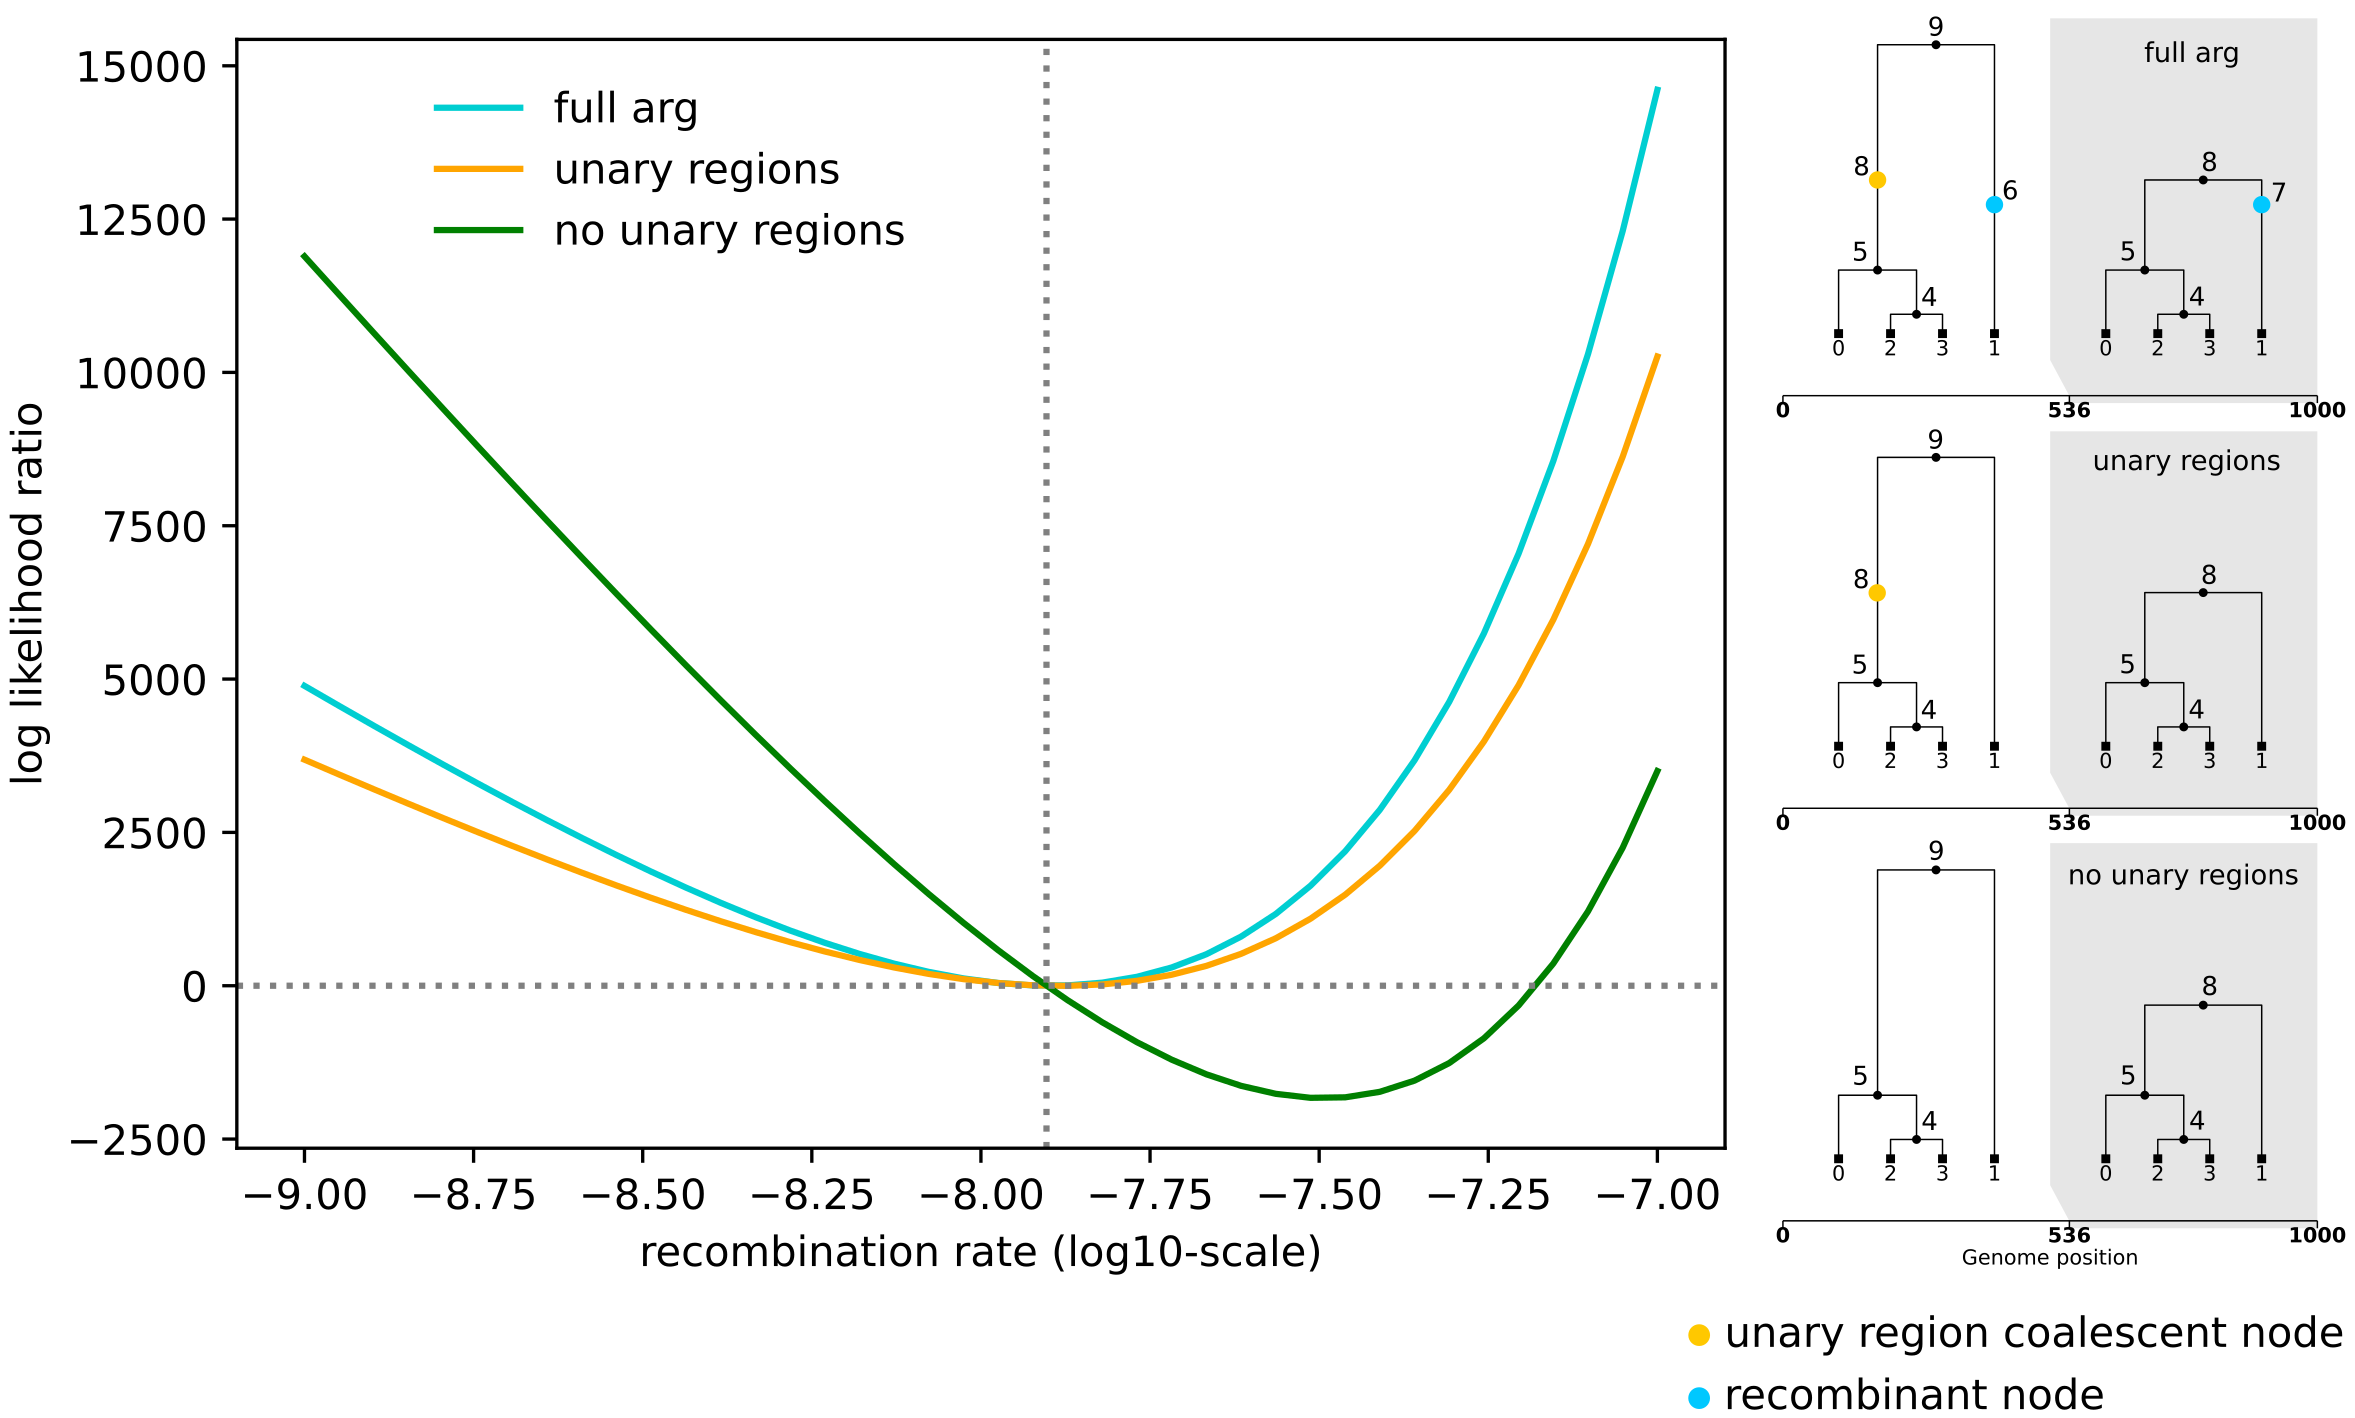
\includegraphics[width=\textwidth]{figures/likratio.png}
    \caption{Log likelihood-ratio curves for ARGs simulated under the SMC with
    various degrees of completeness. The likelihood ratio is computed with
    respect to the true recombination rate. In case of the full ARG the likelihood
    under the SMC has been computed using the exact time to the recombination event.
    Simulation performed with \texttt{msprime}, parameters: $L=1$Mb, $20$ diploid samples,
    $r=2.5e-8$, $N_e=1e4$.}
    \label{fig:lik-surface}
\end{figure}


% slicing of the ARG
By explicitly associating a single likelihood with each edge,
we can compute the likelihood for any slice of the ARG taken in
time and/or along the genome.
In the case of a fully precise ARG, with a known time to recombination,
this is true as long as the slicing operation does not erase the
information on whether an edge is associated with the lefthand or
righthand segment generated by a recombination event. In the absence
of the exact time to recombination, the integral in
eq.\ \ref{eq:depth} means that the likelihood
for the entire ARG does not factorize into the likelihoods of these
individual slices. More precisely, the likelihood associated with any
edge that is initiated by a recombination breakpoint cannot be factorized
into the product of two integrals of the same form.

However, as long as the individual slices of the ARG contain sufficient
information we can approximate the true integral as the product of the
integral of the slices. Figure \ref{fig:3-arg-slices} demonstrates this idea
on a toy example. We simulated an ARG under human-like parameters with
two effective population size changes, and subsequently computed the posterior
distribution on the three effective population sizes
using a uniform prior on each slice independently.
The result is reasonably accurate, despite only using 10kb of sequence.
This approach therefore strengthens
the inherent ability of ARGs to provide us with temporal
resolution and context to a dataset of genetic variation.
It also opens up the opportunity for more efficient optimization
strategies during inference given that each slice of the ARG can be
processed independently. And it further highlights the flexibility
of the algorithm. Simply stated and from a data structure perspective,
we can compute a likelihood under the SMC for any valid tree sequence.
The \texttt{tskit} library provides a wide range
of subsetting operations on tree sequences allowing us to slice
the ARG in time and/or space, as well as to reduce the number of
tracked samples. Any such subset of the tree sequence is itself
a valid tree sequence for which we can again compute a likelihood.


% Although we can associate a likelihood with any valid tree sequences,
% there are some caveats. By treating each edge independently we can
% naturally deal with the various degrees of completeness to which inheritance
% is documented by the different ARG inference methods: e.g., polytomies, absence
% of locally unary coalescence nodes, unpreserved identify of internal nodes
% across marginal trees, etcetera.
% However, many of these imprecisions violate the implicit
% assumptions of the likelihood computation.
% \comment{Do we want these remarks in here, or as part of the Discussion?}
% 
% For example, the described algorithm assumes the
% presence of ``locally unary'' nodes to correctly identify the
% full extent of all lineages going back through time and therefore recombination events.
% Without unary nodes though, our algorithm will detect a recombination
% event along both coalescing lineages in case of a (sub)tree height changes along
% the ARG as both edges would switch parent nodes. This can be mitigated by limiting
% the number of 'inferrable' recombination events per coalescence event to 1
% (see fig \ref{sup:fig:rec-correction}).
% \comment{I'm not editing this in since I'm not sure I've got it right:
% I think that as written, our algorithm would count an extra recombination
% and and extra coalescence for any edge that got split up by removing the unary bits.
% This could be corrected for in the algorithm, but it would require extra bookkeeping,
% and make the likelihood not so easily a product over edges. (?)}
% 
% \comment{this was previously part of the discussion, have grouped it here.}
% Although their presence is crucial to our ability to embed any local tree in the
% ARG, the concept and their importance are still relatively new (but see
% \citet{wong_general_2023}).
% We have briefly touched upon the observation that in
% the presence of unary nodes we seem to augment the left-to-right logic of the SMC
% with some additional information. Yet, we believe that the topic of locally
% unary nodes in general requires further exploration.
% And more specifically, we see it as future work to fully quantify to what
% extent the absence of these locally unary nodes will affect the shape of the
% likelihood surface given any set of parameters.

%%% remarks on precision of information + useage of likelihood to either
%%% estimate parameters (not goal here) or use as instrument to improve accuracy to infer ARGs

\begin{figure}[!ht]
    \centering
    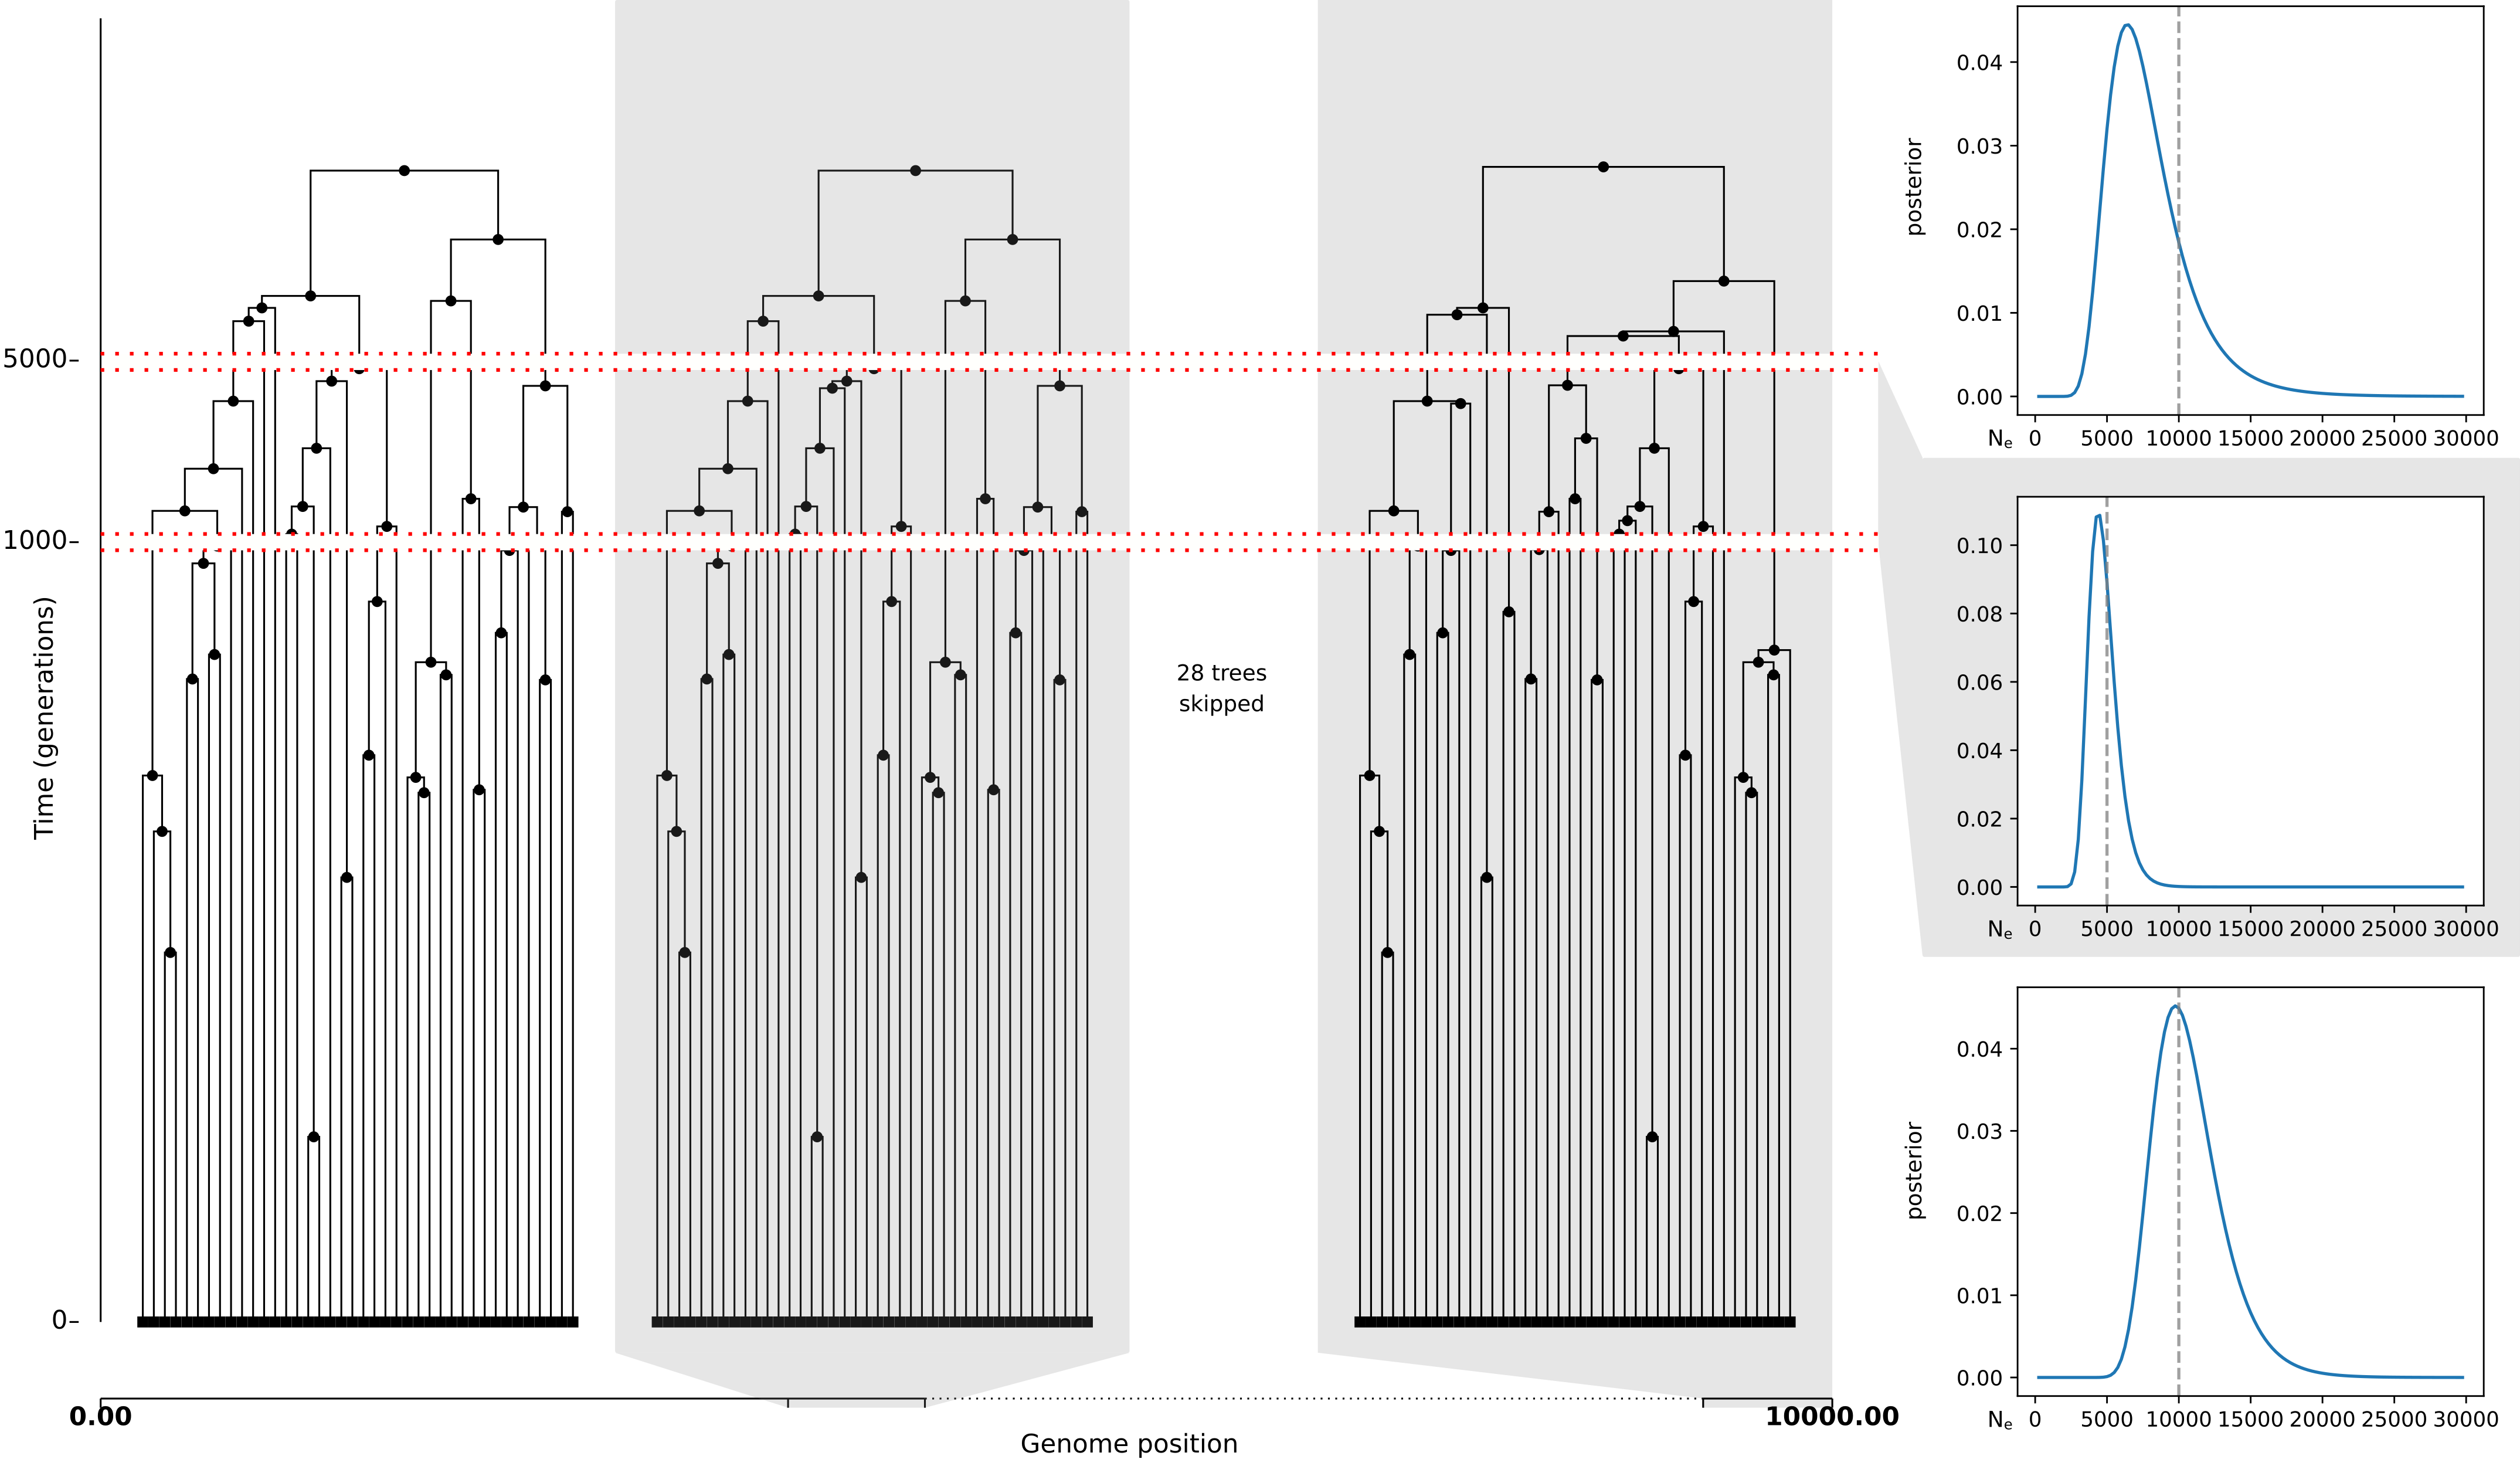
\includegraphics[width=\textwidth]{figures/3-slices-whitespace.png}
    \caption{Simulated ARG under Hudson coalescent (left). $N_e$ is constant
    for each of the 3 time slices: $[(0:1000): 10 000, (1000:5000): 5000,
    (5000:\infty):10 000]$. Remaining parameters: $L=10$kb, $20$ diploid samples,
    $r=2.5e-8$, $148$ edges in ARG. A single $N_e$ value was estimated for each
    slice of the ARG as defined by the true population size change time points.
    The inferred posterior distribution (right) using the SMC-likelihood was
    obtained using a uniform prior. Number of edges per time slice
    (from most recent slice to oldest): $[68, 57, 23]$. Locally unary nodes were
    omitted for clarity.}
    \label{fig:3-arg-slices}
\end{figure}


\section{Discussion}

Here, we have introduced a scalable algorithm to compute likelihoods
under the SMC for a general class of ARGs. By formulating the SMC backwards in time
we were able to associate a single likelihood value with each edge in the ARG.
The compatibility of the algorithm with the \texttt{tskit} library allows us to
exploit its associated efficiencies both for the current work and its future
applications. This work will contribute significantly
to ARG-based analysis becoming a standard part of the population
and statistical genetics toolkit.
In particular, we see two main applications for the work presented here.
Firstly, the ability to associate inferred ARGs with a likelihood given a demographic
model and an associated set of parameters, will help bridge the gap between the tremendous recent
advances in ARG inference and the current state of the art statistical inference of
past demography.
The second and probably the most important application of the ability to associate a more
general class of ARGs to a principled model is the ability to boost the current efforts
in ARG inference. 
% great starting point for MCMC
Any inferred ARG can be used a good starting point
for a future MCMC-sampler. This potentially implies a massive runtime reduction by
reducing the necessary burn-in period. Furthermore, by integrating out the exact time
to the recombination event we further restrict the size of the ARG space that needs to
be explored. This MCMC-sampler would again rely on the tree sequence data structure to
efficiently generate and evaluate any new proposal (see \citep{mahmoudi_bayesian_2022}).
% hybrid ARG-inference: scalability + bringing ARG down from pedigree dominated phase
To further improve scalability, hybrid ARG-inference methods could be designed which
rely on heuristic approaches to bring the ARG down from the initial pedigree-dominated phase,
and subsequently use a principled approach to perform ARG inference for the second phase.
This idea resembles the tried and tested approach of hybrid backwards-in-time simulations 
that combine Wright-Fisher dynamics in the very recent past and coalescent simulations 
for the remaining time \citep{bhaskar_distortion_2014, nelson_accounting_2020}. This hybrid
approach has enabled large scale simulations while avoiding the documented biases of the
coalescent relative to the Wright-Fisher model \citep{bhaskar_distortion_2014, wakeley_gene_2012}. 
The same approach could be thus used for ARG-inference where one can rely on a heuristic 
inference method for the recent past, while using a model-based approach beyond that cutoff point.

Finally, acknowledging the uncertainty associated with ARG inference does not
necessarily require a full-blown MCMC sampler. Instead, recognising those parts of
the ARG for which we lack information for confident reconstruction and resolving
them stochastically by sampling from the coalescent rather than completely arbitrarily
would already be a major step forward. 
% this part is only a very rough idea, might be better to leave it out if we can't make it more concrete.
Furthermore, we believe that quantifying uncertainty
would not necessarily always have to be associated with sampling from the space of all
compatible genealogies. Uncertainty could also
be quantified and passed on as metadata to the nodes in the data format storing the ARG.


%% NOTE: this is some orphan text from the intro that can be rejiggered for the 
% discussion. We can talk about precision of recombination estimates a bit 
% here I think, as it is an important topic.

% Both approaches have further formed the basis (of many) of the recent advancements in
% ARG inference methods \citep{rasmussen_genome-wide_2014, heine_bridging_2018,
% kelleher_inferring_2019, speidel_method_2019, rasmussen_espalier_2022, zhang_biobank-scale_2023}.
% A further classification of these methods could be made based on the level of detail
% that is provided on recombination events. The first real breakthrough in large-scale
% ARG inference, \argweaver, heads the first group.
% The ARGs sampled by \argweaver from the posterior distribution
% given the observed variational data, are all fully precise and detailed in the sense
% that all events are explicitly inferred. Note however that the set of possible node times
% has to be limited to enable the usage of an HMM. The other more recent methods, although
% still SMC-based, have added heuristic pre- and/or post-processing steps
% that have allowed them to extend their approach to larger sample sizes. We should also
% mention \kwarg and \texttt{ARGinfer} in this category of methods producing fully detailed ARGs
% although these are not based on the SMC or the copying algorithm. In fact they represent
% two extremes along the approximation continuum with \kwarg being entirely
% parsimony-based while \texttt{ARGinfer} is a CwR-based MCMC sampler.

%% Recent progress in ARGs through approximate structures}

% The second group of methods (\tsinfer, \relate, \argneedle) has marked a significant
% leap in scalability. These methods derive their scalability at least to a certain
% degree from the fact that the ARGs they infer are approximate structures. In particular,
% recombination is an emergent property of the inferred ARGs, explaining tree topology
% changes going from one local tree to the next. The recombination events themselves
% are not explicitly inferred and are thus not part of the resulting data structure.

% The computational gains from not having to pinpoint recombination events tie in
% with the inevitable uncertainty associated with ARG reconstruction [Hayman, 2022, ADD REFS].
% Some approaches have embraced the approximate nature of the resulting ARG by, for
% example, highlighting the inability to resolve certain splits and instead representing
% them as polytomies \citep{kelleher_inferring_2019}. Taken together this means that the
% degree of completeness in which genetic inheritance from ancestors to descendants is documented
% by each of these methods varies extensively.
% [TO ADD: these methods only provide point estimates]


\section{Data availability}

All scripts and data used for this manuscript are available on https://github.com/gertjanbisschop/smc-bit-paper
An implementation of the algorithm is available on https://github.com/gertjanbisschop/runsmc.
\FloatBarrier
\bibliographystyle{plainnat}
\bibliography{refs.bib,paper.bib}

\pagebreak

\supplementarysection
\section*{Supplementary Information}

% % % % % % % % % % % % % % % % % %
\subsection{Algorithm} \label{par:algo}

\begin{figure}[!ht]
\centering
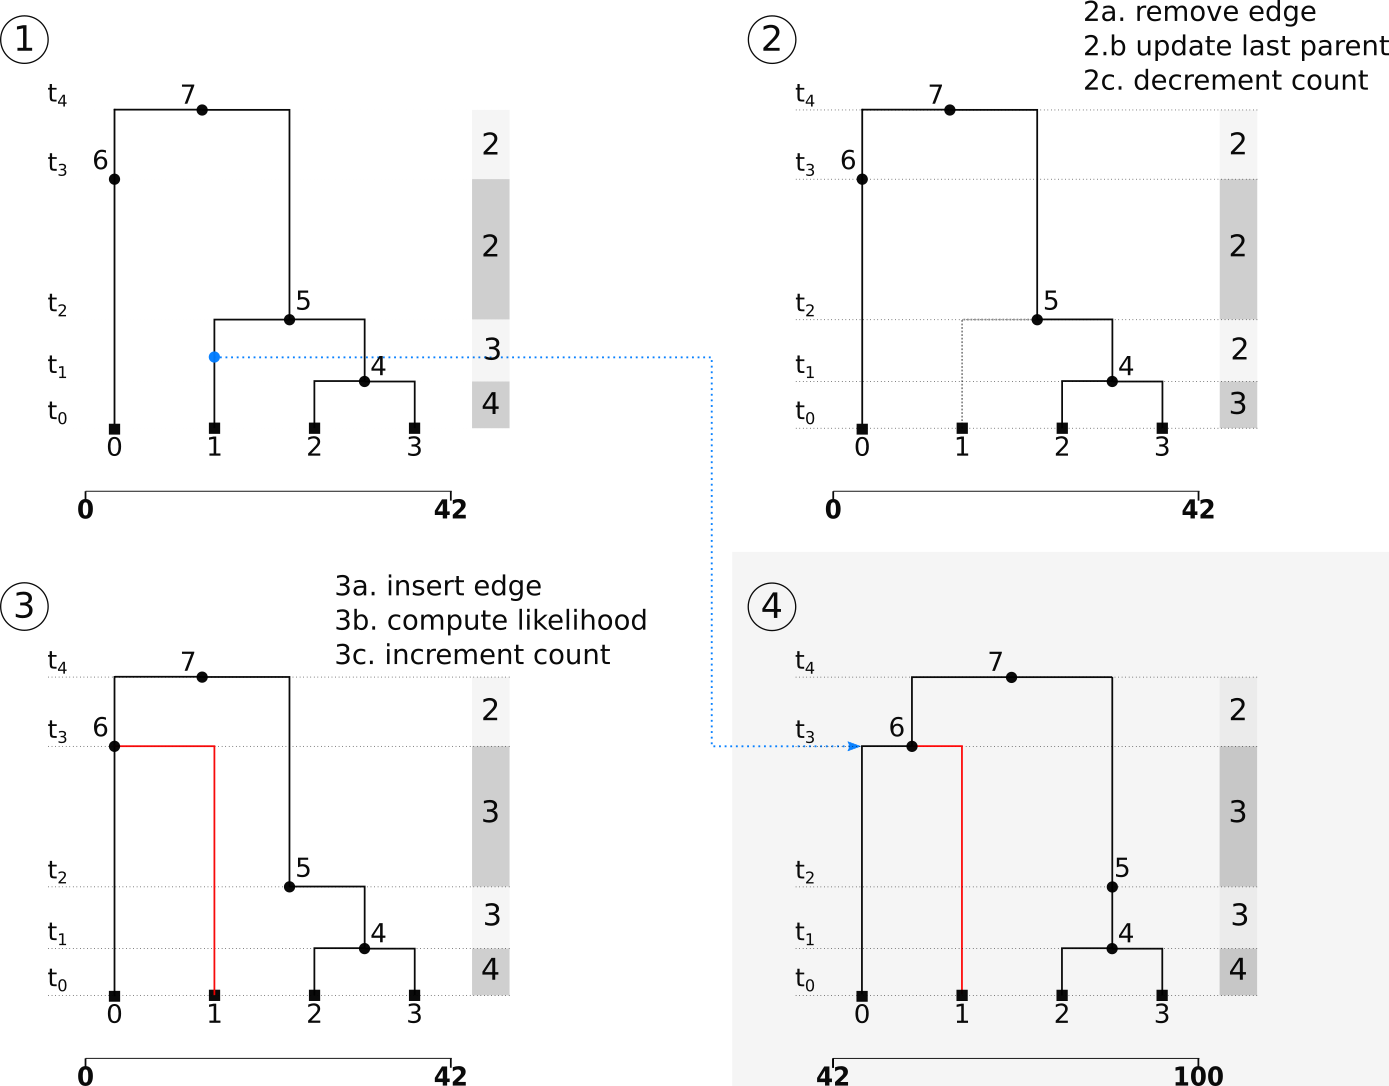
\includegraphics[width=\textwidth]{figures/ts_algo_2rows.png}
\caption{Description of algorithm: Moving along the genome we transition from
local tree $T_1$ to the next, $T_2$ in three steps. 
Edges that do not persist in $T_2$ are
removed first. Edges starting at the left coordinate of $T_2$ are inserted.
After deletion or insertion of an edge the count vector $I$ is updated along the
corresponding internode intervals. Following an insertion, and prior to updating $I$,
the likelihood for that edge is computed as $I$ then represents the total number of
lineages the lineage associated with this new edge can
coalesce with. By moving along the genome in this way, each edge gets visited exactly once.}
\label{fig:algo}
\end{figure}

Next, we describe how to efficiently compute the likelihood under the SMC
from an ARG stored using the \emph{tree sequence} encoding. %  (see fig. \ref{fig:smc-unary}).
The tree sequence format encodes relationships using \emph{edges}
just as described above,
along with additional structure that
allows us to sequentially recover the local trees
along the genome very efficiently, and to reason about
the differences between those trees \citep{kelleher_efficient_2016, ralph_efficiently_2020}.
The order of the edge deletions and insertions required to move from one local tree $T_1$ to
the next, $T_2$ imposes the required strict total ordering on edges
(see definition \ref{def:coal})
that is needed to efficiently maintain the state of $I_e(t)$ for each focal edge $e$.
Indeed, following the removal of edges that do not persist in $T_2$,
we simply declare that each subsequently added edge
can only coalesce with the already-visited edges 
that make up the (partially) reconstructed local tree $T_2$.

This allows us to compute a likelihood in a single pass over all edges.
More concretely, the likelihood is computed by maintaining a single vector $I$ that tracks
the number of extant lineages in each internode interval (see fig \ref{fig:algo}).
When moving from $T_1$ to $T_2$, the vector $I$ is first decremented along the internode intervals
spanned by the time of the child and the parent of all edges that do not persist in $T_2$.
For each subsequently inserted edge, we first compute the likelihood contribution
of that edge by computing the integral
in equation \eqref{eq:full-lik} using $I$, and then update the counts in $I$.
We further keep track of
the last parent a child node was connected to to detect recombination events.

% There is probably no need to potentially confuse people with this detail
%Remark: better to describe edges here as edge-intervals, each describing a
%single contiguous interval of genome inheritance between a pair of nodes.
%Under the SMC and when recording unary nodes all edges can be represented
%by a single edge-interval.

% ADD IN RESULTS:
% Figure \ref{sup:fig:vs-argweaver} shows the expected near-perfect correlation
% between the coalescent prior as returned by \argweaver and the likelihood as computed here.
% We simulated 1Mb of data for 10 diploid individuals
% under the SMC using human-like parameters. 100 samples were taking from the posterior every for
% a total of 1000 MCMC iterations.

% \subsection{Multiple segments description}
% 
% \comment{This is copied from above in case it's helpful in the future.}
% 
% We now define the process more formally,
% and following the notation of \citet{mcvean_approximating_2005}.
% At any point in time, the state of the process is $L(t)$,
% the set of labeled lineages extant at time $t$,
% where each ``lineage'' is represented by a union of non-overlapping half-open intervals
% which represent the ancestral material carried by that lineage,
% and labels are integers.
% So, we can write $L(t) = \{X_i(t)\}_{i=1}^{n(t)}$,
% where the $i^\text{th}$ lineage is $X_i(t)$
% and is of the form
% $X_i(t) = ([x_{i0}, y_{i0}), \dotsc, [x_{im_i}, y_{im_i}))$
% for some interval endpoints $x_{i0} < y_{i0} < x_{i1} < \cdot < y_{im_i}$.
% The \emph{span} of this lineage is the interval $s(X_i(t)) = [x_{i0}, y_{im_i}$,
% and its \emph{size} is $|X_i(t)| = y_{im_i} - x_{i0}$.
% Since we look backwards in time, $t=0$ is today, and so
% $L(0)$ consists of $n$ sampled lineages, labelled $0$ to $n-1$,
% each represented by a single interval spanning the entire genome.
% Then, the process evolves by a succession of coalescence and recombination
% events until each segment of ancestral material is only present in one lineage.
% The waiting time to next event is determined by these two competing processes
% with exponentially distributed waiting times as outlined below.
% 
% Recombination is described by a Poisson process of rate $r$ per unit of genomic length and time:
% so, if $T(t) = \sum_i |X_i(t)|$ is the sum of the total sizes of all lineages,
% then recombination occurs at instaneous rate $rT(t)$.
% A recombination to the left of $x$
% (i.e., between $x$ and $x-1$)
% with $x>x_{i0}$ and $x<y_{im}$ splits lineage $i$ into two new lineages,
% which each are given new, unique labels
% (and lineage $i$ is removed).
% This operation keeps the total amount of ancestral material unchanged.
% 
% Coalescence occurs between
% two lineages with overlapping spans at rate $\lambda = 1/(2N_e)$
% (if we assume a randomly mating, diploid population of constant size $N_e$).
% The newly formed lineage acquires the union of both ordered intervals, % L is updated accordingly
% and the original lineages are removed.
% Although coalescence is reciprocal, here we'll define a strict total order
% on all lineages in $L(t)$ based on their leftmost starting points (and index to break ties).
% For any such strict total order,
% the instantaneous rate of coalescence then equals $\lambda$ multiplied by the number of overlapping pairs,
% i.e., $\lambda \sum_{i \neq j} I_{ij}$,
% where
% \begin{equation}
% I_{ij} = \begin{cases}
%     1 & X_i > X_j \text{ and } s(X_i) \cap s(X_j) \neq \emptyset \\
%     0 & \text{otherwise.}
% \end{cases}
% \end{equation}
% We say that lineage $j$ can coalesce \emph{into} lineage $i$ if $I_{ij} = 1$
% (and notice that if $I_{ij} = 1$ then $I_{ji} = 0$).
% 
% For future use, define $C_i(t)$ to be the set of lineages that can coalesce into lineage $i$,
% i.e., $C_i(t) = \{X_j \in L(t) | I_{ij}(t) = 1\}$.
% (Therefore, $|C_i(t)| = I_{i}(t) = \sum_{j} I_{ij}(t)$.)
% Because $I_{ij}$ is defined in terms of a total order, the sets $C_i(t)$ are disjoint,
% which will simplify the likelihood computations.
% In particular,
% although recombination affects \emph{which} lineages can coalesce into $i$,
% it does not change the \emph{number} of such lineages:
% in other words, a recombination event changes $C_i(t)$ but not $I_{i}$.
% Another useful quantity to know is the number of lineages carrying material
% at each point on the genome:
% for a location $z$ and time $t$, this is
% \begin{equation}
%     N(t,z) = \#\{i : x \le z < y \text{ for some } [x,y) \in X_i(t) \} .
% \end{equation}
% Note that here we are not counting the ``gaps'' in a lineage,
% so that $N(t, z)$ might be less than the number of $i$ with $z \in s(X_i(t))$.
% 
% The recombination and coalescence operations described above
% either split a lineage or merge two overlapping lineages,
% and so as described so far, each lineage will consist of only a single interval,
% rather than a collection of intervals.
% However, there is one more operation:
% when a sub-segment of a lineage is ancestral to all samples,
% that sub-segment is removed.
% Formally, define $Z(t)$ to be the segments on which the lineages have totally coalesced:
% i.e., $Z(t) = \{z : N(t,z) = 1$.
% Then, each coalescence event replaces the resulting lineage $X_i(t)$
% by $X_i(t) \setminus Z(t)$,
% the set of intervals that results from removing $Z(t)$ from all the intervals in $X_i(t)$.
% 
% % note on the disjoint set of intervals for each lineage under the SMC
% Because of this last step, a single lineage can consist of more than one disjoint interval.
% As noted by \cite{mcvean_approximating_2005},
% this implies that the backwards-in-time description of the
% SMC is slightly different from the left-to-right description,
% in which single ancestors only ever span a single segment of genome.
% This is depicted in fig.\ref{fig:smc-unary}:
% for instance, node 8 is ancestral to all samples on the middle two trees.
% However, this does not affect the distribution
% of marginal genealogies up to the roots.
% More precisely, all lineages will be associated with
% a single interval up to the point where one section of the
% genome has reached its most recent common ancestor but the neighbouring parts have not.


\end{document}
